\documentclass[layout=twocolumn]{achemso}

\setkeys{acs}{
	abbreviations = false,
	articletitle  = false,
	keywords      = false,
	maxauthors    = 10,
	super         = true
}

% Comment below before submitting:
\let\titlefont\undefined{}
\usepackage[fontsize=11pt]{scrextend}
\usepackage[hidelinks,colorlinks,citecolor=blue]{hyperref}
%\flushbottom
% Up to this point

\usepackage{amsmath}
\usepackage{amssymb}
\usepackage[T1]{fontenc}
\usepackage{mathtools}
\DeclarePairedDelimiter\set\{\}
%
\usepackage{graphicx}
\DeclareGraphicsExtensions{.pdf,.eps,.png}
\graphicspath{{figures}}
\usepackage[outdir=figures]{epstopdf}
\usepackage{subfig}
\usepackage{xcolor}
%
\usepackage{array}
\newcolumntype{L}{>{$}l<{$}}
\newcolumntype{C}{>{$}c<{$}}
\newcolumntype{R}{>{$}r<{$}}
%
\newcommand{\mt}[1]{\boldsymbol{\mathbf{#1}}}   % matrix symbol
\newcommand{\vt}[1]{\boldsymbol{\mathbf{#1}}}   % vector symbol
\newcommand{\tr}[1]{#1^\text{t}}                % transposition
\newcommand{\diff}[2]{\frac{\partial{#1}}{\partial{#2}}} % derivative
\newcommand{\avg}[1]{\overline{#1}}             % average
\newcommand{\dd}{{\rm d}}  % differential

%\listfiles

\author{Charlles Abreu}
\email{abreu@eq.ufrj.br}
\affiliation{ Chemical Engineering Department, Escola de Quimica, Universidade
    Federal do Rio de Janeiro, Rio de Janeiro, RJ 21941--909, Brazil }

\title{Sparse MBAR}

\abbreviations{i.i.d., MBAR}

\keywords{Free Energy, Reweighting, Multistate, Sparse, Uncertainty}

\begin{document}

%\begin{tocentry}
%Graphical Abstract
%\end{tocentry}

%\tableofcontents

\begin{abstract}
    To be included.
\end{abstract}

\section{Probabilities}\label{sec:probabilities}

Consider a joint probability density of continuous configurations $x$ and discrete thermodynamic states defined by reduced potential functions $u_i(x)$, with $i=1,\dots,K$, given by
\begin{equation}
    \label{eq:joint}
    \rho(i, x) = \omega_i e^{f_i - u_i(x)},
\end{equation}
where $f_i$ is the reduced free energy of state $i$, defined as
\begin{equation}
    f_i = - \ln \int e^{-u_i(x)} dx,
\end{equation}
and $\omega_i$ is an arbitrary importance weight subject to the constraint
$\sum_{i=1}^K \omega_i = 1$.
The marginal distribution of states and the conditional density of configurations given a state are, respectively,
\begin{equation}
    \label{eq:state marginal}
    p(i) = \int \rho(i, x) dx = \omega_i
\end{equation}
and
\begin{equation}
    \label{eq:config given state}
    \rho(x|i) = \frac{\rho(i,x)}{p(i)} = e^{f_i - u_i(x)}.
\end{equation}
where the latter can be recognized as the Boltzmann distribution of state $i$.
The marginal probability distribution of configurations is
\begin{equation}
    \label{eq:config marginal}
    \rho(x) = \sum_{i=1}^K \rho(i, x) = \sum_{i=1}^K \omega_i e^{f_i - u_i(x)}.
\end{equation}
This is a mixture model with $K$ Boltzmann components.
Finally, the conditional probability of states given a configuration is
\begin{equation}
    \label{eq:state given config}
    p(i|x) = \frac{\rho(i,x)}{\rho(x)} = \frac{
        \omega_i e^{f_i - u_i(x)}
    }{
        \sum_{k=1}^K \omega_k e^{f_k - u_k(x)}
    }.
\end{equation}

The expected value of an arbitrary function $g(x)$ is $\mathbb{E}[g(x)] = \int g(x) \rho(x) dx$.
In particular, the expected value of $p(i|x)$ for any target state $i$ is
\begin{equation}
    \label{eq:expectation}
    \mathbb{E}\left[p(i|x)\right] = \int p(i|x) \rho(x) dx = p(i).
\end{equation}

\section{\label{sec:free energy}Free Energy Estimation}

Let $S = \set{(i_n, x_n)}_{n=1}^N$ represent an i.i.d.~sample drawn from a distribution such as that in Eq.~\eqref{eq:joint} but whose free energies are unknown.
We can classify the sample by state, reordering it as $S = \set{S_j}_{j=1}^K$, where $S_j = \set{x_{jn}}_{n=1}^{N_j}$ is the subset of configurations sampled at state $j$, $x_{jn}$ is one of the $N_j$ configurations sampled at state $j$, and $\sum_{j=1}^K N_j = N$.

To estimate the free energies up to an additive constant, we can maximize the log-quasi-likelihood function~\cite{Doss_2014}
\begin{equation}
    \label{eq:log-quasi-likelihood}
    \mathcal{L} = \sum_{n=1}^N \ln p(i_n|x_n)
    = \sum_{j=1}^K \sum_{n=1}^{N_j} \ln p(j|x_{jn}).
\end{equation}

Since $\diff{}{f_i} \ln p(j|x) = \delta_{ij} - p(i|x)$, each condition $\diff{}{f_i} \mathcal{L} = 0$ leads to the equation
\begin{equation}
    \sum_{j=1}^K \sum_{n=1}^{N_j} p(i|x_{jn}) = N_i.
\end{equation}

By undoing the sample reordering, we obtain
\begin{equation}
    \label{eq:maximum quasi-likelihood system}
    \sum_{n=1}^N p(i|x_n) = N_i.
\end{equation}

By substituting Eq.~\eqref{eq:state given config}, we obtain the system of equations
\begin{equation}
    \label{eq:free energy estimators}
    \sum_{n=1}^N \frac{
        \omega_i e^{\hat f_i - u_i(x_n)}
    }{
        \sum_{k=1}^K \omega_k e^{\hat f_k - u_k(x_n)}
    } = N_i.
\end{equation}
for $i=1,\dots,K$, which can be solved numerically for the free energy estimates $\hat f_i$ up to an additive constant.

Interestingly, the state labels $i_n$ serve only to determine $N_i$.
It does not matter which state was initially associated with each configuration~\cite{Kong_2003}.
Eq.~\eqref{eq:maximum quasi-likelihood system} tells us that the free energies which maximize the quasi-likelihood of the sample are the ones that make the estimators $\frac{1}{N} \sum_{n=1}^N p(i|x_n)$ for $\mathbb{E}\left[p(i|x)\right]$ and $\frac{N_i}{N}$ for $p(i)$ mutually consistent.

It is even possible to estimate the free energies without knowing the importance weights $\set{\omega_i}_{i=1}^K$.
Due to Eq.~\eqref{eq:state marginal}, we can substitute $N_i / N$ for $\omega_i$ in Eq.~\eqref{eq:free energy estimators} to obtain
\begin{equation}
    \label{eq:MBAR}
    \sum_{n=1}^N \frac{
        e^{\hat f_i - u_i(x_n)}
    }{
        \sum_{k=1}^K N_k e^{\hat f_k - u_k(x_n)}
    } = 1.
\end{equation}

This is well-known MBAR (Multi-state Bennett Acceptance Ratio) free energy estimator\cite{Shirts_2008}.
There is no difference between the i.i.d.~sample $S$ defined in the beginning of this section and a set of $K$ independent i.i.d.~samples $\set{S_i}_{i=1}^K$, each of which drawn from $\rho(x|i)$, the Boltzmann distribution of configurations at state $i$.

\section{Sparse MBAR}\label{sec:sparse mbar}

The MBAR estimator involves evaluating all $K$ functions $u_i(x)$ for all configurations $x_n$ in the sample.
In certain situations, however, it may be desirable to save computational effort by evaluating only a subset of the functions $u_i(x)$ for each configuration $x$.
Here we propose a sparse MBAR estimator that can be used in such situations.

Let $\mt M$ be a selection matrix such that $m_{ij} = 1$ when evaluation of $u_j(x)$ is available for configurations sampled at state $i$, and $m_{ij} = 0$ otherwise.
We assume that evaluation of $u_i(x)$ will always be available for configurations sampled at state $i$, meaning that $m_{ii} = 1$ for all $i$.
In addition, let $\mathbb{R}_i$ and $\mathbb{C}_i$ be the sets of locations of all non-zero elements in, respectively, the $i$th row and the $i$th column of $\mt M$.
Matrix $\mt M$ is homologous to a directed graph with $K$ nodes, where an edge from node $i$ to node $j$ indicates that evaluation of $u_j(x)$ is available at state $i$.
In this view, $\mathbb{R}_i$ is the set of tails of all edges originating from node $i$ while $\mathbb{C}_i$ the set of heads of all edges terminating at node $i$.
A graphical illustration is shown in Fig.~\ref{fig:directed_graphs}.

\begin{figure}
    \centering
    \subfloat[
        \centering
        $\begin{cases}
            &\color{red} \mathbb{R}_1 = \set{1, 2} \\
            &\color{blue} \mathbb{R}_2 = \set{1, 2, 3, 4} \\
            &\color{orange} \mathbb{R}_3 = \set{2, 3, 4} \\
            &\color{cyan} \mathbb{R}_4 = \set{3, 4}
        \end{cases}$
    ]{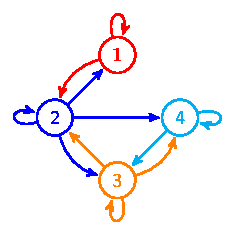
\includegraphics{graph_tails}}
    \subfloat[\centering
        $\begin{cases}
            &\color{red} \mathbb{C}_1 = \set{1, 2} \\
            &\color{blue} \mathbb{C}_2 = \set{1, 2, 3} \\
            &\color{orange} \mathbb{C}_3 = \set{2, 3, 4} \\
            &\color{cyan} \mathbb{C}_4 = \set{2, 3, 4}
        \end{cases}$
    ]{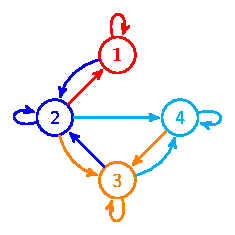
\includegraphics{graph_heads}}
    \caption{Directed graph representation of the selection matrix $\mt M$ and associated sets $\mathbb{R}_i$ and $\mathbb{C}_i$.}\label{fig:directed_graphs}
\end{figure}

Now consider a sampling process restricted to the states of a given subset $\mathbb{R}_i$, according to the joint distribution
\begin{equation}
    \label{eq:subensemble joint}
    \rho_i(j, x) = \omega_{ij} e^{f_j - u_j(x)},
\end{equation}
whose importance weights are subject to the normalization condition $\sum_{j \in \mathbb{R}_i} \omega_{ij} = 1$.
In this case, the conditional probability of states given configurations is
\begin{equation}
    \label{eq:subensemble conditional}
    p_i(j|x) = \frac{
        \omega_{ij} e^{f_j - u_j(x)}
    }{
        \sum_{k \in \mathbb{R}_i} \omega_{ik} e^{f_k - u_k(x)}
    }
    \quad \forall \quad j \in \mathbb{R}_i.
\end{equation}

In the context of MBAR, a subsample $S^\mathbb{R}_i = \set{S_k}_{k \in \mathbb{R}_i}$ detached from $S$ is indistinguishable from an i.i.d.~sample drawn from the distribution in Eq.~\eqref{eq:subensemble joint}.
Unfortunatelly, in a sparse MBAR setup as described above, a conditional $p_i(j|x_{jn})$ cannot be evaluated unless $\mathbb{R}_j \subseteq \mathbb{R}_i$, which is a very restrictive condition.
To cope with this limitation, we propose a log-quasi-likelihood function $\mathcal{L}_s$ in which every state sample $S_j$ is supposed to be part of the subsample $S^\mathbb{R}_j$ rather than the full sample $S$, that is,
\begin{equation}
    \label{eq:sparse log-quasi-likelihood}
    \mathcal{L}_s = \sum_{j=1}^K \sum_{n=1}^{N_j} \ln p_j(j|x_{jn}).
\end{equation}

Before we proceed, we note that any sum over a set $\mathbb{R}_j$ or $\mathbb{C}_j$ can be expressed as a sum over all states if we scale each summand by the proper element of the selection matrix $\mt M$.
These identities make it easier to derive the gradient of $\mathcal{L}_s$ with respect to the free energies $f_i$, which is found to be
\begin{multline}
    \label{eq:sparse gradient}
    \diff{\mathcal{L}_s}{f_i} = \sum_{j=1}^K \sum_{n=1}^{N_j} \left[
        \delta_{ij} - m_{ji} p_j(i|x_{jn}) \right] = \\
    = N_i - \sum_{j \in \mathbb{C}_i} \sum_{n=1}^{N_j} p_j(i|x_{jn}).
\end{multline}

As we do not know the importance weights $\omega_{ij}$, we must replace them by their importance-sampling estimates $\hat{\omega}_{ji} = N_i/\sum_{k \in \mathbb{R}_j} N_k$.
Fortunately, as the denominator in $\hat{\omega}_{ji}$ cancels out, the final system of equations for the free energies turns out to be very similar to the original MBAR estimator.
It is
\begin{equation}
    \sum_{j \in \mathbb{C}_i} \sum_{n=1}^{N_j} \frac{
        e^{\hat{f}_i - u_i(x_{jn})}
    }{
        \sum_{k \in \mathbb{R}_j} N_k e^{\hat{f}_k - u_k(x_{jn})}
    } = 1.
\end{equation}

\section{Conclusion}

%\begin{acknowledgement}
%    The authors acknowledge...
%\end{acknowledgement}

\bibliography{main}

\end{document}